\documentclass[12pt, t]{beamer}

%doc
%https://www.kernel.org/doc/pending/hotplug.txt
%http://electronics.stackexchange.com/questions/37814/usart-uart-rs232-usb-spi-i2c-ttl-etc-what-are-all-of-these-and-how-do-th

%------------------------------------------------------------------------------
% configuration
%------------------------------------------------------------------------------
\RequirePackage{etex}
\usepackage{currfile-abspath}
\usepackage{../../themes/dbt}
\usepackage{catchfilebetweentags}

\setbeameroption{hide notes}
\setbeamertemplate{caption}{\raggedright\insertcaption\par}

\graphicspath{{images/}}
\getmainfile
\getabspath{\themainfile}
\let\mainabsdir\theabsdir
\let\mainabspath\theabspath

\newcommand{\insertcode}[2]{\lstinputlisting[label=samplecode, basicstyle=#1]{\mainabsdir/code/#2}}
\newcommand{\bi}{\begin{itemize}}
\newcommand{\ei}{\end{itemize}}
\newcommand{\ig}{\includegraphics}
\newcommand{\myhref}[1]{\href{#1}{\tt \scriptsize #1}}
\newcommand{\incnote}[1]{\note{\ExecuteMetaData[notes.tex]{#1}}}
\newcommand{\src}[2]{\vspace{-10pt}\caption{\href{#1}{\centering \tt \tiny [#2]}}}


%------------------------------------------------------------------------------
% title
%------------------------------------------------------------------------------
%------------------------------------------------------------------------------
% title
%------------------------------------------------------------------------------
% slide
\title{Systèmes d'exploitation pour l'embarqué}
\subtitle{UV 5.2 - Exécution et Concurrence}

\author{\href{}{Paul Blottière}}
\institute{
    \href{http://www.ensta-bretagne.fr/}{ENSTA Bretagne} \\[2pt]
    \href{}{\tt \scriptsize 2017 / 2018}
}
\date{
    \href{https://github.com/pblottiere}{\tt \scriptsize https://github.com/pblottiere} \\[2pt]
    %\href{blottiere.paul@gmail.com}{\tt \scriptsize blottiere.paul@gmail.com}
}

% info
\begin{document}

{
\setbeamertemplate{footline}{} % no page number here
\frame{
    \titlepage
} }

%------------------------------------------------------------------------------
% amélioration continue
%------------------------------------------------------------------------------
\begin{frame}{Amélioration continue}
    \subt{Contributions}
    \vspace{12pt}

    \begin{center}
    
\includegraphics[scale=0.7]{github.png}
    \end{center}

    \bi
    \itemsep12pt
    \item Dépôt du cours : \href{https://github.com/pblottiere/embsys}{\tt \scriptsize https://github.com/pblottiere/embsys}
    \item Souhaits d'amélioration, erreurs, idées de TP, ... : ouverture d'Issues (avec le bon label!)
    \item Apports de corrections : Pull Request
    \ei
\end{frame}




%<**lecture_content>
%------------------------------------------------------------------------------
% lecture
%------------------------------------------------------------------------------
\begin{frame}[plain,c]
    \centering
    \huge\textcolor{title}{Linux : bus et communication}
\end{frame}

%------------------------------------------------------------------------------
% plan
%------------------------------------------------------------------------------
\begin{frame}{Plan}
    \subt{}
    \vspace{20pt}

    \begin{enumerate}
        \itemsep18pt
        \item Matériel et filesystem
        \item Bus d'extension PCI
        \item GPIO
        \item Port parallèle
        \item Bus CAN
        \item Les bus séries
    \end{enumerate}

    \note {
    }
\end{frame}

%------------------------------------------------------------------------------
% fs1
%------------------------------------------------------------------------------
\defverbatim{\lstdev}
{
    \begin{lstlisting}
> ls /dev
...          dvd        ...
cdrw         dvdrw
cdrom        fb0
...          fb1
    \end{lstlisting}
}

\begin{frame}{Matériel et filesystem (1)}
    \subt{/dev}

    \vspace{20pt}
    Le répertoire /dev (comme \textit{device}) contient des fichiers spéciaux
    permettant notamment d'accèder aux éléments matériels de la machine.

    \onslide<2->
    {
        \vspace{20pt}
        \lstdev

        \centering
        \myhref{http://www.linux-france.org/article/grl/Guide\_Rootard-12.html}
    }
\end{frame}

%------------------------------------------------------------------------------
% fs2
%------------------------------------------------------------------------------
\defverbatim{\lstproc}
{
    \begin{lstlisting}
> ls /proc/bus
input pci
> ls/proc/bus/pci
00  01  09  0a  10  devices
    \end{lstlisting}
}

\begin{frame}{Matériel et filesystem (2)}
    \subt{/proc}

    \vspace{20pt}
    Système de fichiers virtuels {\textit{procfs}} qui contient quelques
    informations sur la configuration matérielle en plus des paramètres
    logiciels du noyau.

    \vspace{20pt}
    \lstproc

\end{frame}

%------------------------------------------------------------------------------
% fs3
%------------------------------------------------------------------------------
\begin{frame}{Matériel et filesystem (3)}
    \subt{/sys}

    \vspace{20pt}
    Relativement récent dans le kernel Linux : version 2.6.x.

    \onslide<2->
    {
        \vspace{20pt}
        Système de fichiers virtuels {\textit{sysfs}} géré par le kernel et
        fournissant des informations basiques sur les périphériques connectés
        au système.
    }

    \onslide<3->
    {
        \vspace{20pt}
        A l'époque, /dev était statique ({\textbf{mknod}}). Désormais, des
        utilitaires comme udev ou mdev scan /sys et peuple le /dev dynamiquement.
    }

\end{frame}

%------------------------------------------------------------------------------
% fs4
%------------------------------------------------------------------------------
\begin{frame}{Matériel et filesystem (4)}
    \subt{/sys}

    \vspace{10pt}
    Le kernel notifie l'espace utilisateur lors de l'insertion grâce au
    mécanisme de {\textit{hotplug}}.

    \onslide<2->
    {
        \vspace{5pt}
        \begin{figure}
            \centering
            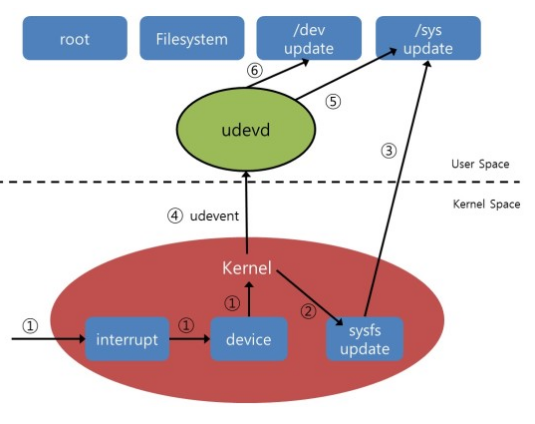
\includegraphics[scale=0.5]{udev.png}
            \src{http://hoonycream.tistory.com/entry/udev}{udevd}
        \end{figure}
    }

\end{frame}

%------------------------------------------------------------------------------
% fs5
%------------------------------------------------------------------------------
\begin{frame}{Matériel et filesystem (5)}
    \subt{/sys}

    \vspace{15pt}
    Dans les systèmes embarqués :
    \vspace{5pt}
    \bi
    \itemsep12pt
    \item mdev (de busybox) est davantage utilisé que udev sur les petits
          systèmes (démon udevd peut consommer plus d'1 MB de RAM).
    \item le mécansime de hotplug peut être désactivé.
    \ei

    \vspace{10pt}
    \begin{figure}
        \centering
        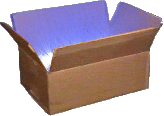
\includegraphics[scale=0.5]{busybox.png}
    \end{figure}

\end{frame}

%------------------------------------------------------------------------------
% pci1
%------------------------------------------------------------------------------
\begin{frame}{Bus d'extension PCI (1)}
    \subt{Description}

    \vspace{15pt}
    {\textbf{ISA}} : Industry Standard Architecture / IBM / années 1980

    \vspace{15pt}
    {\textbf{PCI}} : Peripheral Component Interconnect / Intel / années 1990
                     (half duplex)

    \vspace{15pt}
    {\textbf{AGP}} : Accelerated Graphics Port / Intel / années 1990

    \vspace{15pt}
    {\textbf{PCIe}} : PCIexpress / Intel / années 2000 (full duplex)

    \onslide<2->
    {
        \vspace{15pt}
        => spécification de bus interne permettant la connexion de cartes
        d'extension sur la carte mère.
    }
\end{frame}

%------------------------------------------------------------------------------
% pci2
%------------------------------------------------------------------------------
\begin{frame}{Bus d'extension PCI (2)}
    \subt{Exemples}

    \begin{figure}
        \centering
        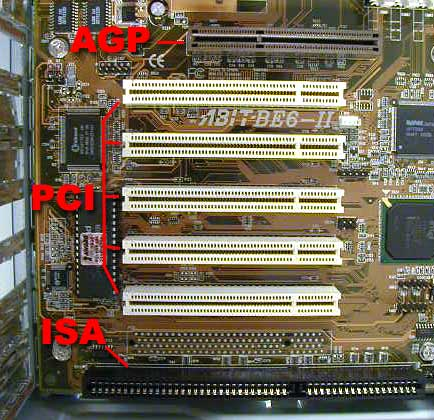
\includegraphics[scale=0.4]{agp-or-pci-or-isa.jpg}
    \end{figure}

\end{frame}

%------------------------------------------------------------------------------
% pci3
%------------------------------------------------------------------------------
\begin{frame}{Bus d'extension PCI (3)}
    \subt{Exemples}

    \begin{figure}
        \centering
        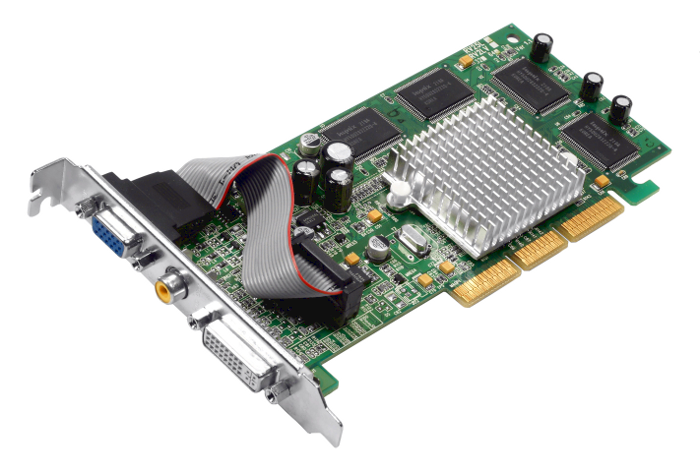
\includegraphics[scale=0.35]{graphic-card.png}
    \end{figure}

\end{frame}

%------------------------------------------------------------------------------
% pci4
%------------------------------------------------------------------------------
\begin{frame}{Bus d'extension PCI (4)}
    \subt{Exemples}

    \begin{figure}
        \centering
        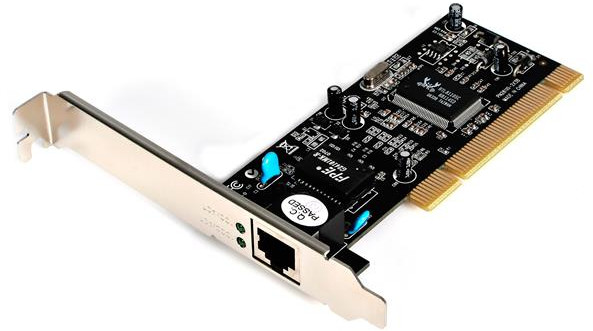
\includegraphics[scale=0.5]{network-card.jpg}
    \end{figure}

\end{frame}

%------------------------------------------------------------------------------
% pci5
%------------------------------------------------------------------------------
\begin{frame}{Bus d'extension PCI (5)}
    \subt{Bridge}

    \vspace{10pt}
    Certaines cartes d'extension doivent pouvoir communiquer entre elles. Cela
    est réalisé par l'intermédiaire d'un {\textit{bridge}}.

    \begin{figure}
        \centering
        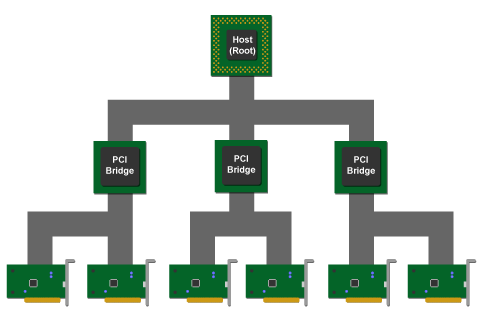
\includegraphics[scale=0.5]{pci-bridges.png}
    \end{figure}

\end{frame}

%------------------------------------------------------------------------------
% pci6
%------------------------------------------------------------------------------
\begin{frame}{Bus d'extension PCI (6)}
    \subt{Adressage}

    \vspace{5pt}
    Un bus PCI est défini sous Linux par quatre numéros :
    \bi
    \itemsep5pt
    \item domaine : 16 bits
    \item bus : 8 bits
    \item port : 5 bits
    \item fonction : 3 bits
    \ei

    \onslide<2->
    {
        \vspace{10pt}
        La commande {\textbf{lspci}} peut être utilisée pour lister le matériel
        PCI : carte d'extension, bridge ou controller.
    }

    \onslide<3->
    {
        \vspace{10pt}
        [man] : {\textit{Some  parts  of  the  output,  especially in the
        highly verbose modes, are probably intelligible only to experienced PCI
        hackers. For exact definitions of the fields, please consult either the
        PCI specifications or the header.h and /usr/include/linux/pci.h include
        files.}}
    }

\end{frame}

%------------------------------------------------------------------------------
% pci7
%------------------------------------------------------------------------------
\defverbatim{\lstlspci}
{
    \begin{lstlisting}[basicstyle=\scriptsize]
> lspci
00:00.0 Host bridge: Intel Corporation 2nd Generation Core
        Processor Family DRAM Controller (rev 09)
00:01.0 PCI bridge: Intel Corporation Xeon E3-1200/2nd
        Generation Core Processor Family PCI Express Root
        Port (rev 09)
00:1a.0 USB controller: Intel Corporation 6 Series/C200
        Series Chipset Family USB Enhanced Host Controller
00:1b.0 Audio device: Intel Corporation 6 Series/C200 Series
        Chipset Family High Definition Audio Controller (rev 05)
00:1f.0 ISA bridge: Intel Corporation HM65 Express Chipset
        Family LPC Controller (rev 05)
01:00.0 VGA compatible controller: Advanced Micro Devices,
        Inc. [AMD/ATI] Seymour [Radeon HD 6400M/7400M Series]
09:00.0 Network controller: Broadcom Corporation BCM4313
        802.11bgn Wireless Network Adapter (rev 01)
10:00.0 Ethernet controller: Qualcomm Atheros AR8151 v2.0
        Gigabit Ethernet (rev c0)
\end{lstlisting}
}

\begin{frame}{Bus d'extension PCI (7)}
    \subt{lspci}

    \vspace{15pt}
    \lstlspci

\end{frame}

%------------------------------------------------------------------------------
% pci8
%------------------------------------------------------------------------------
\defverbatim{\lstsys}
{
    \begin{lstlisting}[basicstyle=\scriptsize]
ls /sys/bus/pci/devices/0000\:09\:00.0/
broken_parity_status  consistent_dma_mask_bits  dma_mask_bits
enable                index                     local_cpulist
msi_bus               power                     reset
subsystem             uevent                    class
d3cold_allowed        driver                    firmware_node
irq                   local_cpus                net
remove                resource                  subsystem_device
vendor                config                    device
driver_override       ieee80211                 label
modalias              numa_node                 rescan
resource0             subsystem_vendor
    \end{lstlisting}
}

\begin{frame}{Bus d'extension PCI (8)}
    \subt{udevadm}

    \begin{figure}
        \centering
        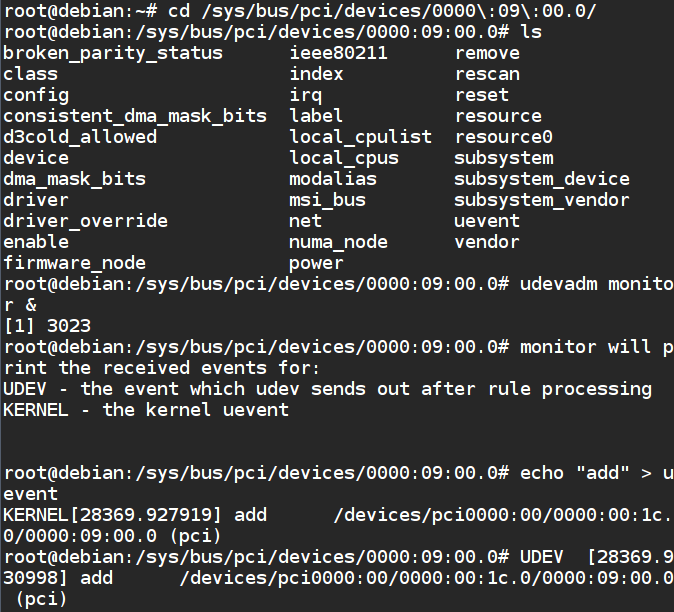
\includegraphics[scale=0.45]{udevadm.png}
    \end{figure}

\end{frame}

%------------------------------------------------------------------------------
% gpio1
%------------------------------------------------------------------------------
\begin{frame}{GPIO (1)}
    \subt{Principe}

    \vspace{20pt}
    GPIO : General Purpose Input/Output (1980)

    \vspace{20pt}
    Purement numérique (1 ou 0).

    \vspace{20pt}
    Souvent de tension 3v3 et de faible courant (de 3mA à 50mA)

    \vspace{20pt}
    Très utilisé : trigger, interruption, led, ...

\end{frame}

%------------------------------------------------------------------------------
% gpio2
%------------------------------------------------------------------------------
\begin{frame}{GPIO (2)}
    \subt{Raspberry Pi}

    \vspace{10pt}
    \begin{figure}
        \centering
        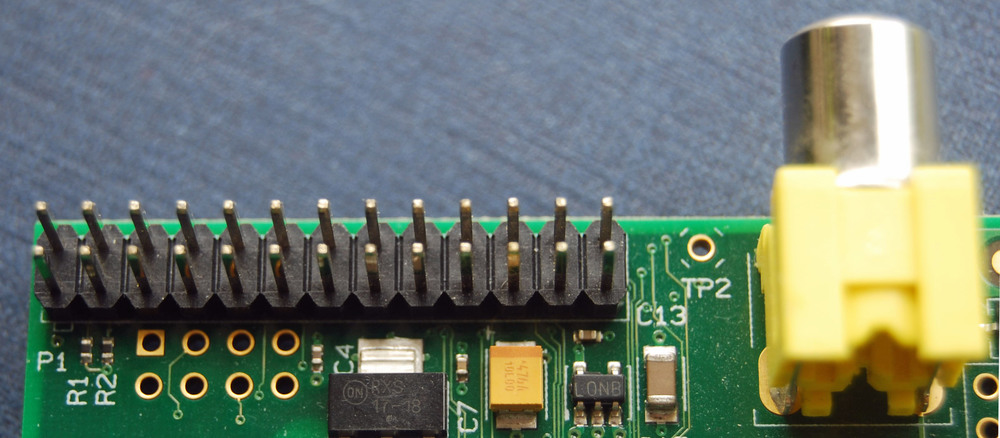
\includegraphics[scale=0.6]{gpio-pins.jpg}
    \end{figure}

    \begin{figure}
        \centering
        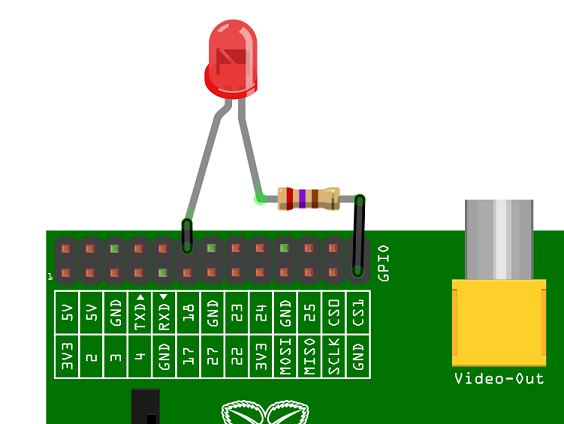
\includegraphics[scale=0.4]{gpio-led.png}
    \end{figure}

\end{frame}

%------------------------------------------------------------------------------
% gpio3
%------------------------------------------------------------------------------
\defverbatim{\lstsysgpio}
{
    \begin{lstlisting}
> cd /sys/class/gpio
> ls
export    unexport
> echo 18 > export
export    gpio18    unexport
> cd gpio18
> ls
active_low  direction   edge    subsystem    uevent    value
> cat direction
in
> echo out > direction
> cat value
0
> echo 1 > value
    \end{lstlisting}
}

\begin{frame}{GPIO (3)}
    \subt{De l'espace utilisateur}

    \vspace{3pt}
    Dans l'espace utilisateur, les GPIOs sont accessibles à travers /sys :
    \vspace{3pt}

    \onslide<2->
    {
        \lstsysgpio
    }

\end{frame}

%------------------------------------------------------------------------------
% gpio4
%------------------------------------------------------------------------------
\defverbatim{\lstconfgpio}
{
    \begin{lstlisting}[basicstyle=\scriptsize]
> cat /boot/config-4.2.0-1-amd64 | grep GPIO_SYSFS -B 13 -A 1
#
# Pin controllers
#
# CONFIG_DEBUG_PINCTRL is not set
# CONFIG_PINCTRL_AMD is not set
# CONFIG_PINCTRL_BAYTRAIL is not set
# CONFIG_PINCTRL_CHERRYVIEW is not set
# CONFIG_PINCTRL_SUNRISEPOINT is not set
CONFIG_ARCH_WANT_OPTIONAL_GPIOLIB=y
CONFIG_GPIOLIB=y
CONFIG_GPIO_DEVRES=y
CONFIG_GPIO_ACPI=y
# CONFIG_DEBUG_GPIO is not set
# CONFIG_GPIO_SYSFS is not set
    \end{lstlisting}
}

\begin{frame}{GPIO (4)}
    \subt{De l'espace utilisateur}

    \vspace{10pt}
    Pour avoir accès aux GPIOs à travers /sys, il faut que le kernel soit
    configuré pour.

    \onslide<2->
    {
        \vspace{10pt}
        Example de kernel non configuré :
        \vspace{5pt}
        \lstconfgpio
    }

\end{frame}

%------------------------------------------------------------------------------
% gpio5
%------------------------------------------------------------------------------
\begin{frame}{GPIO (5)}
    \subt{De l'espace kernel}

    \vspace{15pt}
    Depuis l'espace kernel, un module peut avoir accès aux broches en
    lecture/écriture grâce aux appels :

    \vspace{10pt}
    \bi
    \itemsep8pt
    \item gpio\_get\_value
    \item gpio\_set\_value
    \item gpio\_request
    \item gpio\_direction\_input
    \item gpio\_direction\_output
    \item ...
    \ei

\end{frame}

%------------------------------------------------------------------------------
% para1
%------------------------------------------------------------------------------
\begin{frame}{Port parallèle (1)}
    \subt{Principe}

    \vspace{20pt}
    Port parallèle unidirectionnel : 1980

    \vspace{20pt}
    Port parallèle bidirectionnel : 1990

    \vspace{20pt}
    Communication octet par octet (transmission simultanée de 8 bits).

    \vspace{20pt}
    Notamment utilisé par les périphériques type imprimante (/dev/lpX).

\end{frame}

%------------------------------------------------------------------------------
% para2
%------------------------------------------------------------------------------
\begin{frame}{Port parallèle (2)}
    \subt{Connecteur DB25}

    \vspace{15pt}
    Côté connecteur, un port parallèle est représenté par un DB25 :

    \begin{figure}
        \centering
        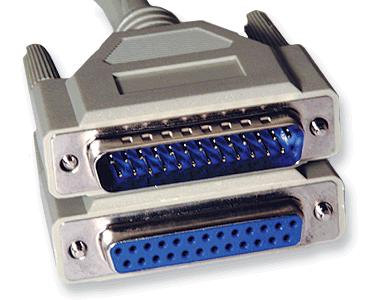
\includegraphics[scale=0.25]{db25.jpeg}
    \end{figure}

    \onslide<2->
    {
        \begin{figure}
            \centering
            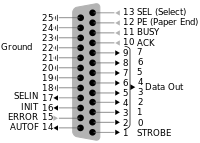
\includegraphics[scale=0.7]{db25-pinout.png}
        \end{figure}
    }

\end{frame}

%------------------------------------------------------------------------------
% para3
%------------------------------------------------------------------------------
\begin{frame}{Port parallèle (3)}
    \subt{Port à tout faire}

    \vspace{15pt}
    Le DB25 est souvent utilisé comme un melting pot d'entrées/sorties sans
    lien avec la communication parallèle.

    \onslide<2->
    {
        \begin{figure}
            \centering
            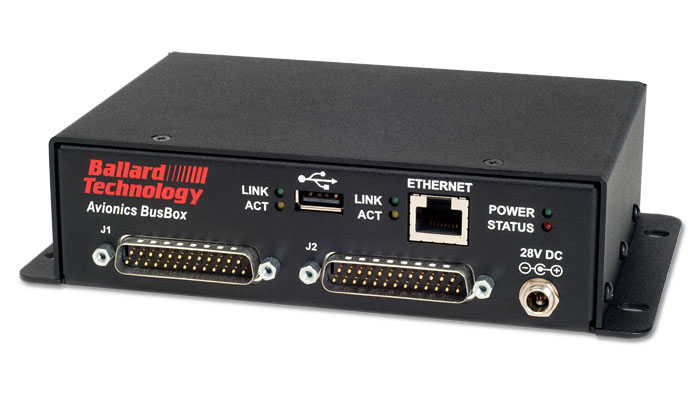
\includegraphics[scale=0.35]{ballard.jpg}
        \end{figure}
    }

\end{frame}

%------------------------------------------------------------------------------
% serial1
%------------------------------------------------------------------------------
\begin{frame}{Communication série (1)}
    \subt{Principe}

    \vspace{15pt}
    Contrairement à la communication parallèle, le protocole série envoie
    des informations bit par bit.

    \onslide<2->
    {
        \vspace{15pt}
        \begin{figure}
            \centering
            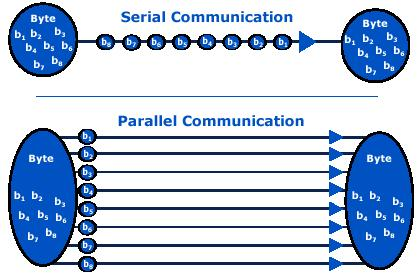
\includegraphics[scale=0.5]{serial_vs_para.jpeg}
        \end{figure}
    }

    \onslide<3->
    {
        => on a alors un multiplexage de type TDM (Time Division Multiplexing)
    }

\end{frame}

%------------------------------------------------------------------------------
% serial2
%------------------------------------------------------------------------------
\begin{frame}{Communication série (2)}
    \subt{Description}

    \vspace{15pt}
    Les avantages de la liaison série par rapport à la communication parallèle :
    \bi
    \itemsep5pt
    \item moins de diaphonie (induction électromagnétique)
    \item skew moins important (différence de temps de propagation)
    \ei

    \onslide<2->
    {
        \vspace{15pt}
        Il existe de nombreux types de liaison/bus série :
        \bi
        \itemsep5pt
        \item RS232 / RS422 / RS485 / RS423
        \item I2C
        \item USB
        \item et d'autres encore (SPI, TTL, ...)
        \ei
    }
\end{frame}

%------------------------------------------------------------------------------
% serial3
%------------------------------------------------------------------------------
\begin{frame}{Communication série (3)}
    \subt{RS232}

    \vspace{7pt}
    Au minimum 3 fils sont nécessaires pour ce type de communication : c'est une
    liaison point à point non différentielle full-duplex (RX / TX / GND).

    \onslide<2->
    {
        \vspace{7pt}
        Il existe plusieurs types de brochage permettant d'exploiter ou non la
        totalité des fonctionnalités du protocole comme le handshaking ou le
        contrôle de flux.
    }

    \onslide<3->
    {
        \vspace{7pt}
        \begin{figure}
            \centering
            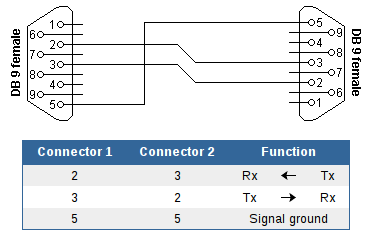
\includegraphics[scale=0.6]{rs232-db9.png}
        \end{figure}
    }
\end{frame}

%------------------------------------------------------------------------------
% serial4
%------------------------------------------------------------------------------
\begin{frame}{Communication série (4)}
    \subt{RS232}

    \vspace{5pt}
    Pour réaliser une communication série, un protocole doit être établi :

    \bi
    \item 1 bit de départ
    \item 7 ou 8 bits de données
    \item 1 bit de parité optionnel
    \item 1 ou plusieurs bits d'arrêt
    \ei

    \onslide<2->
    {
        \begin{figure}
            \centering
            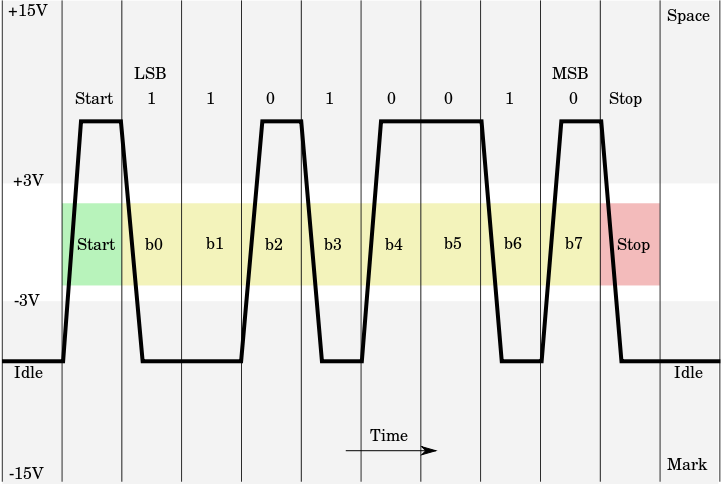
\includegraphics[scale=0.23]{rsr232-k.png}
            \src{https://fr.wikipedia.org/wiki/RS-232\#/media/File:Rs232\_oscilloscope\_trace.svg}{K}
        \end{figure}
    }
\end{frame}

%------------------------------------------------------------------------------
% serial5
%------------------------------------------------------------------------------
\begin{frame}{Communication série (5)}
    \subt{RS232}

    \vspace{10pt}
    Sous Linux, l'API {\textbf{termios}} est utilisée pour gérer les interfaces
    série à travers {\textbf{/dev/ttySx}} dans l'espace utilisateur.

    \onslide<2->
    {
        \vspace{10pt}
        La programmation d'une interface série se fait via :
        \bi
        \itemsep5pt
        \item la structure {\textbf{termios}} : configuration générale (parité,
              contrôle de flux, ...)
        \item {\textbf{cfsetospeed}} / {\textbf{cfsetispeed}} : le débit
        \item {\textbf{tcsetattr}} : mise en place effective de la configuration
        \item {\textbf{fcntl}} : lecture bloquante ou non
        \item {\textbf{open}} / {\textbf{read}} / {\textbf{clos}}e : gestion du
              file descriptor
        \ei
    }

    \onslide<3->
    {
        \vspace{10pt}
        Référence : \myhref{http://tldp.org/HOWTO/Serial-Programming-HOWTO/x115.html}
    }
\end{frame}

%------------------------------------------------------------------------------
% serial6
%------------------------------------------------------------------------------
\begin{frame}{Communication série (6)}
    \subt{I2C}

    \vspace{15pt}
    Inter Integrated Circuit : bus série half-duplex.

    \onslide<2->
    {
        \vspace{15pt}
        La topologie du bus est de type maître esclave où la connexion est réalisée
        via 3 fils :
        \bi
        \itemsep8pt
        \item La masse (GND)
        \item Serial Data Line (SDA) : un signal de données
        \item Serial Clock Line (SCL) : un signal de synchronisation
        \ei
    }
\end{frame}

%------------------------------------------------------------------------------
% serial7
%------------------------------------------------------------------------------
\begin{frame}{Communication série (7)}
    \subt{I2C}

    \vspace{15pt}
    Exemple de montage :
    \begin{figure}
        \centering
        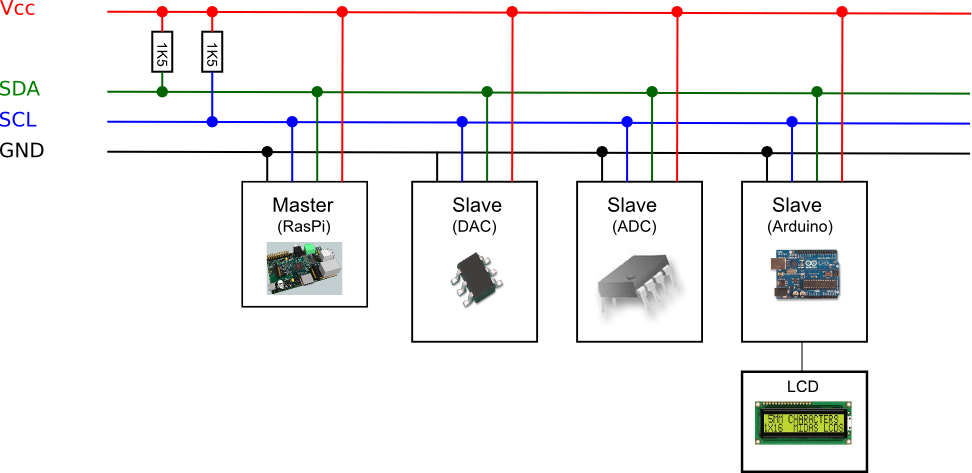
\includegraphics[scale=0.3]{i2c.png}
        \src{http://quick2wire.com/articles/i2c-and-spi/}{Montage I2C}
    \end{figure}

\end{frame}

%------------------------------------------------------------------------------
% serial8
%------------------------------------------------------------------------------
\defverbatim{\lstiic}
{
    \begin{lstlisting}
> sudo modprobe i2c-dev
> cd /sys/class/i2c-dev/
> ls
i2c-0  i2c-1  i2c-10  i2c-11  i2c-12  i2c-13  i2c-14
i2c-2  i2c-3  i2c-4   i2c-5   i2c-6   i2c-7   i2c-8
i2c-9
> cd  i2c-0
> ls
dev  device  name  power  subsystem  uevent
    \end{lstlisting}
}

\begin{frame}{Communication série (8)}
    \subt{I2C}

    \vspace{15pt}
    Depuis l'espace utilisateur, le matériel I2C est accessible à travers /sys
    après chargement d'un module :

    \vspace{10pt}
    \lstiic

\end{frame}

%------------------------------------------------------------------------------
% serial9
%------------------------------------------------------------------------------
\defverbatim{\lstiicopen}
{
    \begin{lstlisting}
int file;
char *filename = "/dev/i2c-2";
if ((file = open(filename, O_RDWR)) < 0) {
    perror("Failed to open the i2c bus");
    exit(1);
}
    \end{lstlisting}
}
\begin{frame}{Communication série (9)}
    \subt{I2C}

    \vspace{20pt}
    Exemple d'ouverture d'un port I2C par flux :
    \vspace{10pt}
    \lstiicopen

\end{frame}

%------------------------------------------------------------------------------
% concl1
%------------------------------------------------------------------------------
\begin{frame}{Conclusion}

    \centering
    \vspace{20pt}
    \LARGE{
        Il existe de très nombreux protocoles de communication et connaître
        les principaux est indispensable.

        \begin{figure}
            \centering
            
\includegraphics[scale=0.5]{socket.png}
        \end{figure}
    }

\end{frame}

%------------------------------------------------------------------------------
% ref
%------------------------------------------------------------------------------
\begin{frame}{Références}
    \vspace{30pt}

    \bi
    \itemsep12pt
    \item https://github.com/torvalds/linux/tree/master/Documentation
    \item https://lwn.net/Kernel/LDD3/
    \item http://tldp.org/HOWTO/Serial-Programming-HOWTO/
    \item Linux Embarqué - Pierre Ficheux
    \ei

\end{frame}
%<//lecture_content>

\end{document}
